\subsubsection{K-Means}
There are many methods by which to cluster, K-Means is a popular method due to its speed and simplicity. Data points are sorted into one of K clusters where the average value of the cluster is stored in a central data point known as the cluster centroid. Centroids may initially be randomly generated or selected from the given data set. 

Data points or samples are placed in the class of the centroid that is closest to them. The distance between them is the Euclidean Distance between their feature vectors as in \ref{eq:euclid}. 

\begin{equation}
    D(\vec{p},\vec{q}) = \sqrt{(p_1 - q_1)^2 + (p_2 - q_2)^2 +\hdots + (p_n - q_n)^2}
    \label{eq:euclid}
\end{equation} 

K-Mean's algorithm proceeds as follows:
    \begin{enumerate}
    \itemsep0em
        \item Place the initial K centroids.
        \item Assign all data points to their nearest centroid.
        \item Update the centroids' values to be the mean of all data points in their cluster.
        \item Repeat steps 2 and 3 until a criteria is met, for example until cluster centroids no longer move (converge).
    \end{enumerate}

K-means benefits greatly from its low computational cost such that it is oten performed a number of times with different initial centroids and the instance best result is used. The best result is defined as having the smallest intracluster variance. K-Means is disadvantaged by the implicit trait that it formulates clusters of similar sizes. This happens because the algorithm seeks to minimize variance (spread) in each cluster hence the \q{ideal} centroid placement will form distributions spherically about centroids. This method cannot disentangle overlapping samples that belong in different classes. In Figure \ref{fig:clusters} clear edges between clusters and sphereical distributions can be observed. The algorithm can only implement \emph{hard assignments}, as opposed to a \emph{soft assignment} that consider the probability of a sample's class membership. 



\begin{figure}[H]
    \centering
    \centering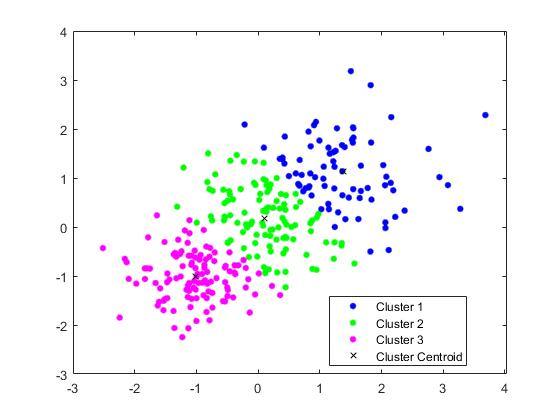
\includegraphics[width=300pt]{kmeans_clusters}
    \caption{K-Means clustering performed on random data.}
    \label{fig:clusters}
\end{figure} 